\documentclass{math}

\usepackage{pgfplots}
\usetikzlibrary{arrows}

\title{Multivariable and Vector Calculus}
\author{Alvin Lin}
\date{August 2017 - December 2017}

\begin{document}

\maketitle

\section*{Quadric Surfaces}
Quadric surfaces are surfaces that can be described by quadratic equations in
\( \R^3 \).
\[ ax^2+by^2+cz^2+dxy+exz+fyz+gx+iy+hz = j \]
We will only consider the cases where the coefficients \( d,e,f \) are zero
and there are no mixed variables.

\subsubsection*{Example}
Sketch \( z = x^2+4y^2 \). Trace:
\[\begin{split}
  z &= 0 \\
  0 &= x^2+4y^2
\end{split}
\quad
\begin{split}
  z &= 1 \\
  1 &= x^2+4y^2
\end{split}
\quad
\begin{split}
  z &= 5 \\
  5 &= x^2+4y^2
\end{split}
\quad
\begin{split}
  z &= -1 \\
  -1 &= x^2+4y^2
\end{split} \]
Starting from \( z = 0 \), this figure is a single point and expands as a series
of ellipses along the positive z axis. If we take a slice along the yz-plane:
\begin{align*}
  x &= 0 \\
  z &= 4y^2
\end{align*}
\begin{center}
  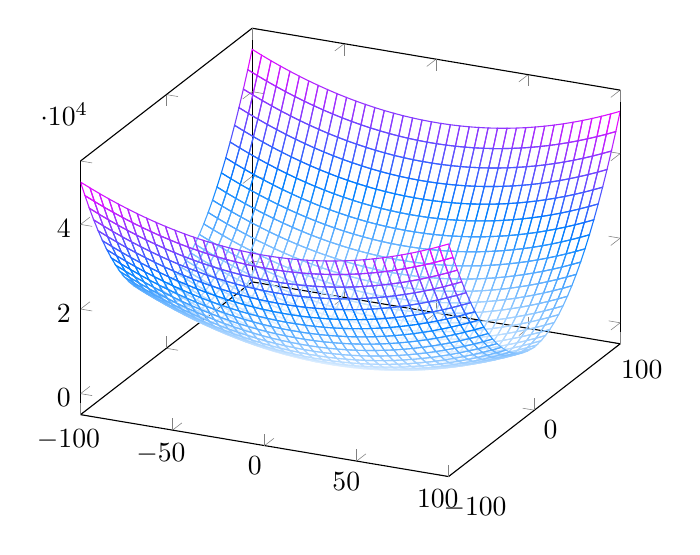
\begin{tikzpicture}
    \begin{axis}[colormap/cool]
      \addplot3[
          mesh,
          samples=40,
          domain=-100:100,
      ]{(x^2)+(4*(y^2))};
    \end{axis}
  \end{tikzpicture}
\end{center}

\subsubsection*{Example}
Sketch \( x^2+4y^2+9z^2 = 9 \):
\[ \begin{split}
  z &= 0 \\
  x^2+4y^2 &= 9
\end{split}\quad\begin{split}
  z &= \pm\frac{1}{3} \\
  x^2+4y^2 &= 8 \\
\end{split}\quad\begin{split}
  z &= \pm1 \\
  x^2+4y^2 &= 0
\end{split}\quad\begin{split}
  x &= 0 \\
  4y^2+9x^2 &= 9
\end{split} \]
This shape is ellipsoidal along the xy-plane.

\subsubsection*{Example}
Sketch \( x^2-4y^2+9z^2 = 9 \):
\[ \begin{split}
  y &= 0 \\
  9 &= x^2+9z^2
\end{split}\quad\begin{split}
  y &= \pm1 \\
  10 &= x^2+9z^2
\end{split}\quad\begin{split}
  y &= \pm5 \\
  109 &= x^2+9z^2
\end{split}\quad\begin{split}
  z &= 0 \\
  x^2-4y^2 &= 9
\end{split} \]
This shape looks like a series of expanding ellipses starting from \( y = 0 \).
It is a hyperboloid.

\subsubsection*{Example}
Sketch \( x^2-4y^2-9z^2 = 9 \):
\[ \begin{split}
  x &= 0 \\
  \emptyset
\end{split}\quad\begin{split}
  x &= \pm3 \\
  0 &= 4y^2+9z^2
\end{split}\quad\begin{split}
  x &= \pm5 \\
  15 &= 4y^2+9z^2
\end{split}\quad\begin{split}
  x &= \pm8 \\
  40 &= 4y^2+9z^2
\end{split}\quad\begin{split}
  x &= 0 \\
  x^2-4y^2 &= 9
\end{split} \]
This shape is a hyperboloid of two sheets.

\subsubsection*{Example}
Sketch \( z^2 = x^2+4y^2 \):
\[ \begin{split}
  z &= 0 \\
  0 &= x^2+4y^2
\end{split}\quad\begin{split}
  x &= \pm1 \\
  1 &= x^2+4y^2
\end{split} \]
This is a series of expanding ellipses starting from \( z = 0 \). If we take
\( x = 0 \), we get \( z^2 = 4y^2 \), which represents two intersecting lines
or the cross section of the ellipses. We know from this that the radii of the
ellipses increase linearly.

\begin{center}
  You can find all my notes at \url{http://omgimanerd.tech/notes}. If you have
  any questions, comments, or concerns, please contact me at
  alvin@omgimanerd.tech
\end{center}

\end{document}
